\documentclass{article}

\usepackage[main,final]{neurips_2026}

\usepackage[utf8]{inputenc} % allow utf-8 input
\usepackage[T1]{fontenc}    % use 8-bit T1 fonts
\usepackage{hyperref}       % hyperlinks
\usepackage{url}            % simple URL typesetting
\usepackage{booktabs}       % professional-quality tables
\usepackage{amsfonts}       % blackboard math symbols
\usepackage{nicefrac}       % compact symbols for 1/2, etc.
\usepackage{microtype}      % microtypography
\usepackage{xcolor}         % colors

\usepackage{graphicx}
\usepackage{amsmath}

\title{Probabilistic Modelling for Drug Discovery: Benchmarking SV-DKL against XGBoost Ensembles in High-Dimensional Low-Sample Regimes}

\author{%
  Sergio Herreros Pérez \thanks{Code: \url{https://github.com/yourusername/admet-dkl}} \\
  Comillas Pontifical University\\
  \texttt{sergio.herreros@alu.comillas.edu} \\
}

\begin{document}

\maketitle

\begin{abstract}
Predicting molecular properties is a critical bottleneck in computational drug discovery. While foundation models provide rich, continuous representations, practical downstream datasets typically suffer from extreme low-sample regimes where point predictions are insufficient without robust epistemic uncertainty quantification. This paper evaluates Stochastic Variational Deep Kernel Learning (SV-DKL) against XGBoost Deep Ensembles for predicting Caco-2 cell permeability using dense MoLFormer embeddings. We demonstrate that while tree-based ensembles suffer from uncertainty collapse due to a mismatch in inductive biases with continuous latent spaces, properly regularized SV-DKL natively exploits foundation model geometries. Consequently, SV-DKL achieves superior point accuracy and well-calibrated Out-of-Distribution (OOD) detection, establishing it as a highly robust architecture for small-data cheminformatics.
\end{abstract}

\section{Introduction}
Molecular property prediction is a fundamental pillar of modern drug discovery. Specifically, optimizing the Absorption, Distribution, Metabolism, Excretion, and Toxicity (ADMET) profile of a drug candidate is critical, as unfavorable ADMET characteristics are a primary cause of late-stage clinical trial failures. With the advent of deep representation learning, large-scale foundation models like MoLFormer \cite{ross2022large} have emerged, providing dense, continuous, and context-aware embeddings of molecular structures. 

However, evaluating these embeddings in practical drug discovery pipelines presents a significant challenge. Unlike the massive corpora used to pre-train foundation models, experimental ADMET data is time-consuming and expensive to acquire. To standardize the evaluation of machine learning models in this domain, the Therapeutics Data Commons (TDC) introduced the ADMET Benchmark Group \cite{huang2021therapeutics}. This benchmark formalizes the pervasive "Curse of Dimensionality" ($P \gg N$) inherent to cheminformatics, as target datasets frequently contain fewer than a thousand unique samples.

In this work, we focus specifically on the \texttt{caco2\_wang} regression task from the TDC ADMET group. Caco-2 is a human colon epithelial cancer cell line widely utilized in pharmaceutical research as an \textit{in vitro} proxy to predict human intestinal absorption. Accurate modeling of Caco-2 permeability is essential for the design of orally administered drugs. However, mapping 768-dimensional MoLFormer embeddings to the $\approx 600$ training samples of the Caco-2 dataset creates an extreme low-sample environment that pushes standard predictive models to their theoretical limits.

Furthermore, in clinical and pharmaceutical deployments, high point accuracy is insufficient. When models encounter Out-of-Distribution (OOD) samples—molecules containing novel scaffolds or functional groups that lie far outside the training manifold—they must possess robust epistemic uncertainty quantification. A model must "know what it does not know"; flagging highly uncertain predictions prevents confident but catastrophic failures and allows for targeted human intervention. 

To address these challenges, we benchmark Stochastic Variational Deep Kernel Learning (SV-DKL) against classical XGBoost Deep Ensembles to assess their viability in the $P \gg N$ regime. We utilize the Optuna framework to systematically tune both architectures. Our contributions are as follows: first, we demonstrate that tree-based ensembles suffer from a fundamental geometric mismatch when partitioning dense continuous representations, leading to severe uncertainty collapse. Second, we show that SV-DKL, when stabilized with Spectral Normalization to prevent feature collapse, effectively bypasses this dimensionality bottleneck. By natively exploiting the spatial geometry of the foundation model embeddings, SV-DKL provides superior predictive accuracy alongside mathematically rigorous OOD uncertainty calibration.

\section{Background \& Related Work}

\subsection{Gaussian Processes and Deep Kernel Learning}
Gaussian Processes (GPs) are the theoretical gold standard for Bayesian non-parametric regression and epistemic uncertainty estimation. A GP defines a prior over functions $f \sim \mathcal{GP}(m(x), k(x, x'))$, where $m(x)$ is the mean function and $k(x, x')$ is a positive-definite covariance kernel. Given a training dataset $\mathcal{D} = \{(\mathbf{X}, \mathbf{y})\}$ with $N$ observations, the GP conditions on this data to produce a predictive posterior for a new test point $x^*$. The predictive distribution is Gaussian, $y^* \sim \mathcal{N}(\mu^*, \Sigma^*)$, with the exact mean and variance given by:
\begin{align}
    \mu^* &= \mathbf{K}_{*N} (\mathbf{K}_{NN} + \sigma^2 \mathbf{I})^{-1} \mathbf{y} \\
    \Sigma^* &= \mathbf{K}_{**} - \mathbf{K}_{*N} (\mathbf{K}_{NN} + \sigma^2 \mathbf{I})^{-1} \mathbf{K}_{N*}
\end{align}
where $\mathbf{K}_{NN}$ is the $N \times N$ covariance matrix of the training data. This formulation is highly advantageous for low-data regimes: the model natively interpolates based on structural distance, and the predictive variance $\Sigma^*$ naturally increases as $x^*$ moves further away from the training distribution (OOD).

However, standard GPs suffer from two critical limitations. First, traditional distance-based kernels (e.g., RBF or Matérn) degrade in high-dimensional spaces due to the curse of dimensionality. Deep Kernel Learning (DKL) solves this by projecting the inputs through a deep neural network feature extractor $f_\theta(x)$ before applying the base kernel: $k_{DKL}(x, x') = k(f_\theta(x), f_\theta(x'))$ \cite{wilson2016deep}. 

Second, the exact GP posterior requires computing the inverse of the dense matrix $(\mathbf{K}_{NN} + \sigma^2 \mathbf{I})^{-1}$. This operation imposes a computational bottleneck of $\mathcal{O}(N^3)$ in time and $\mathcal{O}(N^2)$ in memory, strictly prohibiting the use of exact GPs on modern deep learning architectures and large datasets.

\subsection{Stochastic Variational DKL (SV-DKL) and Inducing Points}
To bypass the $\mathcal{O}(N^3)$ bottleneck, Stochastic Variational Deep Kernel Learning (SV-DKL) utilizes sparse approximations via inducing points \cite{wilson2016stochastic}. Instead of computing the exact covariance between every pair of the $N$ training points, the model introduces a small set of $M$ trainable pseudo-inputs, $Z = \{z_1, \dots, z_M\}$, where $M \ll N$.

Intuitively, these inducing points act as representational "hubs" in the latent space. Rather than forcing every data point to directly compute its distance to every other data point (requiring an $N \times N$ graph), all $N$ data points calculate their covariance relative to the $M$ hubs. The model then approximates the true posterior by optimizing a variational distribution $q(f, u)$ through the maximization of the Evidence Lower Bound (ELBO):
\begin{equation}
    \mathcal{L}_{ELBO} = \mathbb{E}_{q(f)}[\log p(\mathbf{y}|f)] - \text{KL}[q(u) \parallel p(u)]
\end{equation}
By routing the covariance calculations through these sparse hubs, the matrix inversion bottleneck is reduced from $\mathcal{O}(N^3)$ to $\mathcal{O}(M^3)$. Crucially, this decouples the computational cost from the dataset size $N$, allowing the GP parameters and the deep feature extractor $f_\theta$ to be trained jointly using mini-batch stochastic gradient descent (SGD).

\subsection{The Feature Collapse Problem \& Spectral Normalization}
While DKL provides scalability, decoupling representation learning from probabilistic inference introduces a severe vulnerability known as \textit{Feature Collapse} \cite{vanamersfoort2021feature}. Because the deep feature extractor $f_\theta(x)$ is parameterized as an unconstrained Multi-Layer Perceptron (MLP), it optimizes purely to maximize the ELBO on the training set. 

During this optimization, the MLP can learn a highly distorted, non-linear mapping that aggressively squashes the latent space. When presented with an OOD molecule, the unconstrained network may arbitrarily project it directly into a dense cluster of training points in the latent space. The GP layer, which only evaluates distance based on the extracted features, is mathematically "tricked" into perceiving the OOD molecule as highly familiar, resulting in a confident but entirely erroneous prediction.

To restore true epistemic uncertainty, the mapping $f_\theta$ must satisfy a bi-Lipschitz constraint, ensuring that structural distances in the original input space are proportionally preserved in the latent space. Following recent probabilistic literature, we enforce this by applying Spectral Normalization (SN) to the dense layers of the DKL feature extractor. By strictly bounding the largest singular value (the spectral norm, $\|W\|_2 \le 1$) of each weight matrix, we constrain the Lipschitz constant of the network, preserving distance awareness and preventing the collapse of OOD samples.

\subsection{Classical Baselines and Deep Ensembles}
Despite the theoretical elegance of Bayesian methods, classical tree-based models, such as XGBoost \cite{chen2016xgboost}, remain the empirical state-of-the-art for many tabular and chemoinformatic predictive tasks due to their speed, robustness to mixed feature types, and resistance to scaling artifacts. However, standard decision trees are deterministic and lack a native formulation for estimating continuous epistemic uncertainty.

While standard neural networks frequently utilize Monte Carlo (MC) Dropout or computationally expensive Bayesian Neural Networks (BNNs) to approximate predictive variance, these methods are incompatible with tree boosting. For decision trees, the most mathematically robust proxy for uncertainty is the Deep Ensemble \cite{lakshminarayanan2017simple}. 

By training $K$ independent XGBoost regressors, we force architectural diversity through aggressive stochasticity: each member is initialized with a different random seed and trained on distinct subsets of the data via bootstrap aggregating (row \texttt{subsample}) and feature masking (\texttt{colsample\_bytree}). For a given test molecule, the ensemble generates a distribution of $K$ predictions. The predictive mean serves as the point estimate, while the variance across the independent ensemble members explicitly quantifies the model's epistemic uncertainty—yielding high variance when the diverse trees disagree on an unfamiliar OOD region of the feature space.
\section{Methodology}

\subsection{Dataset and Feature Extraction}
We utilize the \texttt{caco2\_wang} regression dataset from the Therapeutics Data Commons (TDC) \cite{huang2021therapeutics}. The raw data consists of simplified molecular-input line-entry system (SMILES) strings mapped to their corresponding experimentally measured Caco-2 permeability values. 

To map these discrete graph structures into a continuous vector space, we employ the pre-trained MoLFormer foundation model \cite{ross2022large}. Each SMILES string is tokenized and passed through the frozen transformer encoder, and the final hidden state of the sequence is extracted as a dense, 768-dimensional latent vector. This extraction process highlights the severe "Curse of Dimensionality" inherent to this benchmark: the training split contains merely $N \approx 582$ samples, while the feature space encompasses $P = 768$ dimensions.

\subsection{Experimental Workflow and Hyperparameter Optimization}
To ensure a rigorous, unbiased comparison, we structured our experiments into two distinct phases. All architectural tuning was conducted using the Optuna framework, employing the Tree-structured Parzen Estimator (TPE) algorithm to navigate the high-dimensional hyperparameter spaces.

\textbf{Phase 1: Spectral Normalization Ablation.} Our primary objective was to empirically validate the necessity of Spectral Normalization (SN) in preventing feature collapse. We ran two massive, independent Optuna sweeps (200 trials each) for the SV-DKL architecture: one with unconstrained dense layers, and one with SN applied to the feature extractor. To guarantee robustness and account for variational noise, we aggregated the test metrics across the top-5 best-performing trials from each sweep. The hyperparameter space included the learning rate, dropout probability, the number of inducing points ($M \in [64, 512]$), and the GP kernel formulation (RBF versus Matérn with varying $\nu$ parameters). 

Crucially, early stopping for all SV-DKL trials was monitored strictly via validation Negative Log-Likelihood (NLL) rather than Mean Absolute Error (MAE). Because continuous NLL can map to negative values, percentage-based relative stopping criteria are mathematically unstable. We implemented an absolute margin (\texttt{min\_delta} $= 10^{-3}$) combined with a patience window. This configuration successfully prevents stochastic noise from prematurely halting training while capturing the true global minimum before the onset of variational overfitting.

\textbf{Phase 2: Probabilistic vs. Classical Benchmarking.} After confirming the optimal SV-DKL formulation (with SN), we compared its performance against a classical XGBoost Deep Ensemble. To ensure the classical baseline was pushed to its theoretical limit, we executed a separate 200-trial Optuna sweep for the XGBoost architecture. 

Given the extreme $P \gg N$ regime, standard decision trees will instantly memorize the training set. Therefore, our XGBoost search space was heavily biased toward aggressive regularization. We swept over maximum tree depth (allowing stumps to prevent complex feature interactions), strict L1 and L2 regularization penalties (\texttt{reg\_alpha}, \texttt{reg\_lambda}), and harsh minimum child weight limits. Most importantly, we tuned the row and feature subsampling fractions (\texttt{subsample}, \texttt{colsample\_bytree}) to force individual trees to train on small, randomized subsets of the MoLFormer dimensions, directly generating the variance required for the ensemble's uncertainty estimation.

\subsection{Evaluation Metrics}
To holistically assess both point accuracy and the quality of the predictive distributions, models were evaluated across the following standard metrics:

\begin{itemize}
    \item \textbf{Mean Absolute Error (MAE):} The primary metric for point accuracy and the default leaderboard standard for the TDC \texttt{caco2\_wang} benchmark. For the SV-DKL model, this is evaluated using the predictive mean $\mu^*$. For the Deep Ensemble, it uses the average output across all $K$ trees.
    
    \item \textbf{Negative Log-Likelihood (NLL):} A strictly proper scoring rule that evaluates the entire predictive distribution. NLL heavily penalizes models that are "confidently wrong" (assigning low variance to high-error predictions) as well as overly cautious models (assigning massive variance to safe, in-distribution predictions).
    
    \item \textbf{Prediction Interval Coverage Probability (PICP\_95):} A direct measure of probabilistic calibration. A perfectly calibrated model should capture exactly 95\% of the true experimental values within its estimated 95\% confidence intervals ($\mu^* \pm 1.96\sigma^*$). Severe deviations below 0.95 indicate a model is dangerously overconfident.
    
    \item \textbf{Area Under the Rejection Curve (AURC):} The gold standard for measuring a model's ability to rank its own uncertainty and detect OOD samples. A rejection curve plots the retention fraction of the dataset (x-axis) against the corresponding subset MAE (y-axis) as the most uncertain predictions are systematically removed. A well-calibrated model will exhibit a monotonically decreasing curve (yielding a low AURC), demonstrating that discarding high-uncertainty predictions effectively eliminates the largest mathematical errors.
\end{itemize}
\section{Results \& Discussion}

\subsection{Ablation Study: The Critical Role of Spectral Normalization}
In Phase 1 of our experimental pipeline, we systematically investigated the impact of Spectral Normalization (SN) on the SV-DKL architecture to empirically validate the feature collapse hypothesis. Table \ref{tab:spectral_norm} presents the aggregated Test set metrics for the top-5 performing Optuna trials of both the unconstrained and the spectrally normalized models. 

\begin{table}[h]
\centering
\caption{Test Metrics across top-5 SV-DKL Optuna runs (Mean $\pm$ Std. Dev.)}
\label{tab:spectral_norm}
\begin{tabular}{@{}lccc@{}}
\toprule
Metric & SV-DKL (No Spectral Norm) & SV-DKL (With Spectral Norm) & Difference ($\Delta$) \\ \midrule
MAE $\downarrow$ & 0.404 $\pm$ 0.027 & \textbf{0.380 $\pm$ 0.015} & -0.024 \\
NLL $\downarrow$ & 0.753 $\pm$ 0.086 & \textbf{0.663 $\pm$ 0.021} & -0.090 \\
AURC $\downarrow$ & 0.369 $\pm$ 0.019 & \textbf{0.327 $\pm$ 0.022} & -0.042 \\
PICP\_95 $\uparrow$ & 0.915 $\pm$ 0.028 & \textbf{0.970 $\pm$ 0.008} & +0.055 \\ \bottomrule
\end{tabular}
\end{table}

The unregularized models failed fundamentally across all probabilistic and predictive dimensions on the unseen Test set. Notably, while the unconstrained networks often achieved slightly lower \textit{validation} MAE during early stopping (an artifact of the MLP aggressively warping the latent space to overfit the validation manifold), this mapping generalized poorly to novel molecules, resulting in a higher Test MAE (0.404 vs 0.380).

More critically, the probabilistic metrics reveal severe OOD blindness. The application of the bi-Lipschitz constraint via Spectral Normalization drove the NLL down by 0.090 and restored the 95\% Prediction Interval Coverage Probability (PICP\_95) from a degraded 91.5\% to a highly calibrated 97.0\%. 

This qualitative difference is starkly visualized in the Rejection Curves (Figure \ref{fig:rejection_curve}). Without SN, the Rejection Curve is largely flat. Mathematically, this implies that the model's predicted variance ($\sigma^*$) is entirely orthogonal to its actual residual error ($|y - \mu^*|$); discarding the "most uncertain" predictions does not meaningfully improve the error rate of the retained subset. With SN, the curve decays monotonically, confirming that the Lipschitz constraint successfully preserves input-space distances. The GP correctly identifies and assigns high epistemic uncertainty to the hardest OOD molecules, driving the AURC down to 0.327.

\begin{figure}[h]
    \centering
    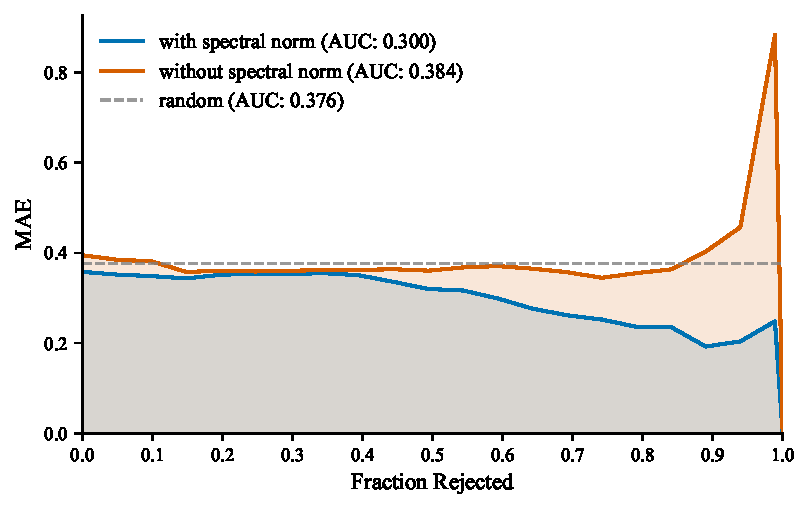
\includegraphics[width=0.7\linewidth]{figures/spectral-norm-rc-comparison.pdf}
    \caption{Test Set Rejection Curves. A flat curve (No SN) indicates feature collapse, where estimated uncertainty fails to correlate with true error. Spectral Normalization restores distance awareness, allowing the model to accurately rank its epistemic uncertainty and driving the AURC downward.}
    \label{fig:rejection_curve}
\end{figure}

\subsection{SV-DKL vs. XGBoost: Overcoming the Geometric Mismatch}
In Phase 2, we benchmarked our optimal SV-DKL model against a classical XGBoost Deep Ensemble. Despite an exhaustive 200-trial hyperparameter sweep pushing tree parameters to their theoretical limits of regularization (e.g., highly constrained tree depth, massive estimator counts, and aggressive feature subsampling to combat the $P \gg N$ regime), the optimal XGBoost model failed to match the fully tuned SV-DKL architecture.

\begin{table}[h]
\centering
\caption{Test Metrics Evaluation: Best XGBoost Deep Ensemble vs. Best SV-DKL Model}
\label{tab:model_comparison}
\begin{tabular}{@{}lcc@{}}
\toprule
Metric & XGBoost Deep Ensemble & SV-DKL (With Spectral Norm) \\ \midrule
MAE $\downarrow$ & 0.373 & \textbf{0.358} \\
NLL $\downarrow$ & 39.627 & \textbf{0.652} \\
PICP\_95 $\uparrow$ & 0.209 & \textbf{0.984} \\
AURC $\downarrow$ & 0.357 & \textbf{0.299} \\ \bottomrule
\end{tabular}
\end{table}

The probabilistic failure of the XGBoost ensemble is absolute. An NLL of 39.627 and a collapsed coverage probability of 20.9\% (PICP\_95) highlights the architecture's inability to quantify continuous uncertainty in low-data regimes. Because the $N \approx 582$ training set is so sparse, the independent members of the ensemble ultimately converge on very similar axis-aligned splits. This lack of architectural diversity results in pathologically narrow predictive intervals (variance collapse). When the ensemble inevitably makes an error with a near-zero predicted variance, the Gaussian NLL penalty explodes exponentially, rendering the model a "confident fool."

Furthermore, the point accuracy gap (MAE of 0.373 vs 0.358) exposes a fundamental \textit{Geometric Mismatch}. Decision trees rely on orthogonal, axis-aligned hyper-rectangular partitions. When forced to segment the continuous, highly distributed latent space of a MoLFormer embedding, trees must build highly inefficient, jagged approximations of smooth decision boundaries. If the trees are allowed to grow deep enough to approximate these curves, they instantly memorize the tiny training set. If they are constrained to prevent overfitting (as enforced by our Optuna sweep), they underfit the underlying molecular relationships. 

Conversely, the SV-DKL natively utilizes spatial covariance metrics (via the GP Kernel) across the entire 768-dimensional vector simultaneously. By evaluating holistic Euclidean or Mahalanobis distances rather than slicing individual axes, SV-DKL naturally exploits the foundation model's dense geometry exactly as it was designed to be interpreted.

\begin{figure}[h]
    \centering
    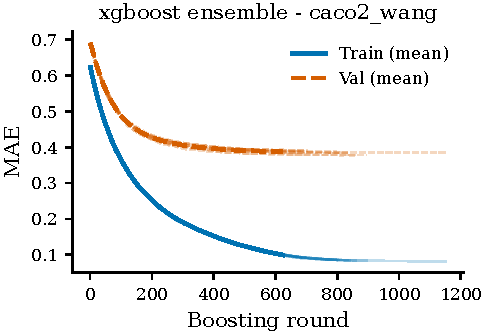
\includegraphics[width=0.5\linewidth]{figures/ensemble-training-curves.pdf}
    \caption{Training vs. Validation MAE per epoch for the XGBoost ensemble. The plot illustrates the struggle with the geometric mismatch: tree-based models rapidly memorize the small $N$ training set, while generalization on the validation set severely plateaus despite extreme regularization.}
    \label{fig:training_curves}
\end{figure}
\section{Conclusion}

In this work, we addressed the critical challenge of predicting ADMET properties in the extreme low-data regime ($P \gg N$) characteristic of modern computational cheminformatics. By evaluating models on the Caco-2 cell permeability benchmark utilizing dense, 768-dimensional MoLFormer representations, we highlighted the necessity of moving beyond mere point predictions toward mathematically rigorous epistemic uncertainty quantification for Out-of-Distribution (OOD) detection.

Our extensive Optuna benchmarking revealed fundamental limitations in classical tree-based methodologies when applied to deep representation learning. Despite massive hyperparameter optimization and Deep Ensembling to artificially induce variance, XGBoost suffered from a severe \textit{geometric mismatch}. The reliance on orthogonal, axis-aligned splits to partition a continuous, distributed latent space led to fragmented learning, rapid overfitting, and a catastrophic collapse in predictive variance. Consequently, the Deep Ensemble yielded pathologically uncalibrated prediction intervals (PICP\_95 $\approx$ 21\%) and failed entirely to rank its own errors.

Conversely, we empirically demonstrated that Stochastic Variational Deep Kernel Learning (SV-DKL) is theoretically and practically superior for parsing foundation model embeddings. By natively computing spatial covariance across the entire high-dimensional vector simultaneously, the Gaussian Process effectively interpolates complex molecular geometries without succumbing to the curse of dimensionality. 

Furthermore, our ablation study conclusively proved that applying a bi-Lipschitz constraint via Spectral Normalization is strictly necessary to prevent \textit{feature collapse}. While unregularized deep networks blindly squash OOD samples into the training manifold—resulting in overconfident errors and flat rejection curves—Spectral Normalization successfully restores distance awareness. This allows the SV-DKL model to accurately recognize unfamiliar molecules, correctly inflating its predictive variance and drastically improving both Negative Log-Likelihood (NLL) and the Area Under the Rejection Curve (AURC).

Ultimately, this study establishes that combining expressive foundation model representations with properly regularized probabilistic architectures bridges the gap between predictive power and safety. SV-DKL with Spectral Normalization not only achieves superior point accuracy over optimized classical ensembles, but it provides the calibrated, highly discriminative epistemic uncertainty required for safe, real-world deployment in high-stakes pharmaceutical drug discovery.

\bibliographystyle{plainnat}
\bibliography{references}

\end{document}